\subsection{Time Constant Calibration Error}

\paragraph{Description:}
Whichever method we use to estimate the time constants of our detectors, an error in this estimate can induce a signal when the incorrect estimate is deconvolved. We describe the transfer function of the detector as $H(\omega)$ in the frequency domain:

\begin{equation}
\label{tc_transfer}
H(\omega, \tau) = \frac{1}{1 + i \omega \tau},
\end{equation}
where, as mentioned in this section's introduction, $\tau = 1/2 \pi f_{\mbox{\scriptsize 3dB}}$. We can now describe the effect of applying the inverse transfer function in both amplitude and phase. If we assume that our measured optical power fluctuations $\delta P$ have been filtered by $H(\omega, \tau_e)$, we apply an inverse transfer function with the measured time constant plus an error term, $H^{-1} (\omega, \tau_e + \Delta \tau)$, where $\Delta \tau$ represents an additive error to the true value $\tau_e$. We recover an absolute square amplitude of power fluctuations $\delta P'$ which relates to the input $\delta P$ as:

\begin{equation}
\label{amp_correct_approx}
|\delta P'|^2 = (1 + \frac{2 \omega^2 \Delta \tau \tau_e + ...}{1 + \omega^2 \tau_e^2}) |\delta P|^2.
\end{equation}
The ellipsis here indicates extended terms in a binomial expansion, which we do not find necessary when comparing this approximation to the full model (see Fig. \ref{tau_miscal}). In phase, the error in the time constant causes the estimated optical power fluctuations to lead the true value by a frequency-dependent phase with the following approximate form:
\begin{equation}
\label{phase_correct_approx}
arg(\delta P') = \omega \Delta \tau / (1 + \omega^2 \tau_e^2).
\end{equation}

In the end, these corrections will affect signals only at very high frequencies, or equivalently covering small scales on the sky. They will also have an effect on the detector noise models generated to perform optimal mapmaking. Where the expectation is that, after correction, the detector power spectral density (PSD) will be completely flat (i.e. white noise) up to high frequencies, the miscalibration results in PSDs which increase or decrease to $(\frac{\Delta \tau}{\tau_e})^2$ times the white noise level as $\omega$ goes to $\infty$.

\begin{figure}[h!]
\centering
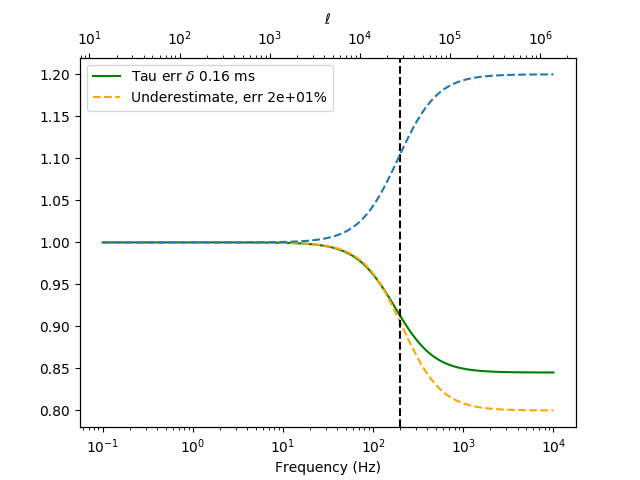
\includegraphics[width=0.4\textwidth]{figures/tau_ampl_error_800us_20pError.png}\quad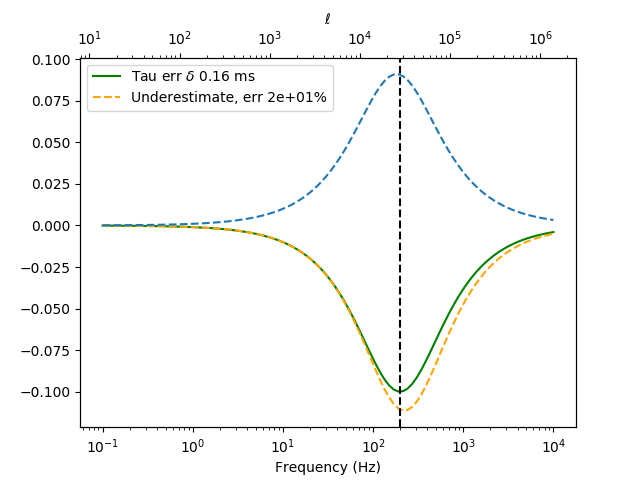
\includegraphics[width=0.4\textwidth]{figures/tau_phase_error_800us_20pError.png}
\caption{0.8ms time constant, 20\% error in estimate. Approximation is solid, dashed is exact numerical. The ideal case would be a flat line at 1.0 vs. frequency for the left panel, and a flat line at 0.0 for the right.}
\label{tau_miscal}
\end{figure}

\paragraph{Plan to model and/or measure:}
SRF = 3. Using a null test of fast vs. slow detectors is a clear indicator of whether time constant miscalibration effects have caused errors in signal estimates. This is also important to determine whether correcting for the transfer function of slower detectors, which affect values of $\ell$ more likely to be of interest than those with larger $f_{\mbox{\scriptsize 3dB}}$, have affected these scales. On a separate note, for the bias step method of measuring time constants, which we expect to be useful as a calibrator as it was in Advanced ACTPol, slower time constants are more easily measured, and will have a smaller absolute error. However, it is possible their fractional errors will remain unchanged, affecting the noise model similarly across detectors.

\paragraph{Uncertainty/Range:}
Errors in time constants can be parametrized in the bias step method using the spread of time constant measurements within a single calibration run. These values are not reported or used for further analysis thus far, but will be studied. Furthermore, their effects on final science products must be investigated to determine whether the current errors set by the various methods are sufficiently stringent. Again, as these effects are only relevant near and above $f_{\mbox{\scriptsize 3dB}}$, especially in amplitude, fast detectors may not need to have their filter functions corrected very accurately in absolute terms.

\paragraph{Parameterization:}
Not yet determined. Could define some ``whiteness criterion'' for the corrected PSD which is acceptable for science work, and target ranges of miscalibration/calibration uncertainty for time constants which meets it. This would need to care about any add-on effects from other detector-based effects on the signals, as well as the estimated $\tau$ values of the detectors while performing CMB observations.